\documentclass[11pt,a4paper]{article}

\usepackage[utf8]{inputenc}
\usepackage[margin=1in]{geometry}
\usepackage{amsmath,amssymb,amsfonts}
\usepackage{graphicx}
\usepackage{booktabs}
\usepackage{multirow}
\usepackage{array}
\usepackage{microtype}
\usepackage{cite}
\usepackage{url}
\usepackage[colorlinks=true,linkcolor=blue,citecolor=blue,urlcolor=blue]{hyperref}
\usepackage{caption}
\usepackage{subcaption}
\usepackage{float}
\usepackage{xcolor}

\title{\textbf{Cross-Cohort and Cross-Platform Evaluation of Stable, Calibrated Gene-Expression Signatures for Estrogen Receptor Status Prediction in Breast Cancer}}

\author{
  \textbf{Kunniyur Ramchander Gautam}\textsuperscript{1,*}, 
  \textbf{Collaborating Investigators}\textsuperscript{1} \\
  \small\textsuperscript{1}Independent Bioinformatics Research Laboratory \\
  \small\textsuperscript{*}Corresponding Author: \href{mailto:research@rapid-er.bio}{research@rapid-er.bio}
}
\date{November 2026}

\begin{document}

\maketitle

\begin{abstract}
\noindent\textbf{Background:} Estrogen receptor alpha ($\text{ER}\alpha$, encoded by \textit{ESR1}) is the paramount predictive biomarker guiding endocrine therapy in breast cancer. Although immunohistochemistry (IHC) remains the routine diagnostic standard, it suffers from documented pre-analytical variability, inter-observer subjectivity, and 5--10\% borderline ambiguity. Transcriptomic profiling provides an orthogonal, objective diagnostic modality. However, previous genomic classifiers frequently suffer from gene-selection instability, cross-platform decay, and severe probability miscalibration under domain shift---a phenomenon we term the \textit{discrimination-calibration paradox}.

\noindent\textbf{Methods:} We established an end-to-end, leakage-free bioinformatics framework (\textbf{RAPID-ER}) across 4,218 audited breast cancer patients from three cohorts: TCGA-BRCA ($N = 1,044$, primary training and 5-fold cross-validation), GSE96058 / SCAN-B ($N = 3,073$, independent external RNA-seq validation), and GSE42568 ($N = 101$, independent cross-platform Affymetrix microarray validation). We mapped a universal gene space of 17,367 HGNC symbols and developed the \textbf{Stability-Selected Multilayer Perceptron (SS-MLP)}, coupling repeated Elastic-Net subsampling (100 bootstrap resamples per partition, selection threshold $\ge 70\%$) with a regularized deep neural network (256-64 GELU architecture with 0.35/0.25 dropout). We benchmarked SS-MLP against an \textit{ESR1}-only logistic baseline and six machine-learning algorithms across two transfer regimes: Transfer Strategy A (frozen training standardization) and Transfer Strategy B (within-sample relative rank normalization). Calibration was assessed via Brier score decomposition (Reliability, Resolution, Uncertainty), Expected Calibration Error (ECE), and logistic calibration parameters.

\noindent\textbf{Results:} On TCGA-BRCA internal 5-fold cross-validation, SS-MLP achieved an out-of-fold AUROC of 0.9560 [95\% CI: 0.9381, 0.9700], AUPRC of 0.9851 [0.9770, 0.9912], Sensitivity of 92.07\%, Specificity of 93.67\%, Brier score of 0.0675, and ECE of 0.0869, closely matching the \textit{ESR1}-only baseline (AUROC 0.9579 [0.9400, 0.9726], Brier 0.0570, ECE 0.0729). On external RNA-seq validation in GSE96058 ($N = 3,073$), \textit{ESR1}-only discrimination remained high under frozen standardization (AUROC 0.9604 [0.9436, 0.9735]), but suffered catastrophic probability miscalibration (ECE = 0.4290, Intercept = 5.2361, Sensitivity = 58.44\%, leaving 1,177 true ER-positive patients misdiagnosed). In contrast, SS-MLP under Strategy A maintained high discrimination (AUROC 0.9500 [0.9326, 0.9651], Sensitivity 97.74\%) while reducing calibration error more than 10-fold to ECE = 0.0396 and Brier = 0.0396. On cross-platform microarrays (GSE42568, $N = 101$), Strategy A collapsed (\textit{ESR1} Sensitivity 0.0000, Brier 0.6188, ECE 0.6313). Label-free within-sample rank normalization (Strategy B) rescued cross-platform performance, elevating SS-MLP AUROC to 0.7943 [0.7011, 0.8743] and AUPRC to 0.8773, with Brier score dropping to 0.3303. In an \textit{ESR1}-exclusion ablation, SS-MLP retained an AUROC of 0.9608 and AUPRC of 0.9863, establishing downstream transcriptomic diagnostic redundancy. Selective classification with abstention at confidence threshold $\tau = 0.80$ achieved 99.6\% autonomous diagnostic coverage on external RNA-seq with a low selective error rate of 3.92\% (dropping to 2.06\% at $\tau = 0.95$), triage-routing uncertain borderline samples for confirmatory review.

\noindent\textbf{Conclusion:} High discriminative AUC can conceal severe probability miscalibration under domain shift. A compact, stability-selected multi-gene signature paired with rank normalization provides platform-resilient, well-calibrated predictions with transparent uncertainty quantification, providing a rigorous paradigm for automated precision oncology decision support.

\medskip
\noindent\textbf{Keywords:} Breast Cancer, Estrogen Receptor, Transcriptomics, Machine Learning, Stability Selection, Deep Neural Networks, Probability Calibration, Domain Transfer, Uncertainty Quantification.
\end{abstract}

\newpage

\section{Introduction}

Breast cancer is the most frequently diagnosed malignant neoplasm and a leading cause of cancer mortality among women globally \cite{sung2021global}. Approximately 70--80\% of all breast carcinomas express estrogen receptor alpha ($\text{ER}\alpha$), encoded by the \textit{ESR1} gene located on chromosome 6q25.1. In clinical oncology, ER status represents the paramount predictive and prognostic biomarker, dictating eligibility for endocrine therapies---including selective estrogen receptor modulators (e.g., tamoxifen), selective estrogen receptor degraders (e.g., fulvestrant), and aromatase inhibitors (e.g., letrozole, anastrozole)---which dramatically reduce disease recurrence and breast-cancer-specific mortality \cite{ebctcg2011relevance}.

Current international guidelines from the American Society of Clinical Oncology and College of American Pathologists (ASCO/CAP) recommend establishing ER status via immunohistochemistry (IHC) on formalin-fixed paraffin-embedded (FFPE) core biopsies or surgical resections, defining ER-positivity as $\ge 1\%$ immunoreactive tumour cell nuclei \cite{allison2020estrogen}. Despite universal adoption, clinical IHC is subject to well-documented pre-analytical and analytical sources of discordance. Cold ischemia intervals, variability in FFPE fixation duration, differing antibody clone affinities (e.g., 1D5 vs.\ SP1 vs.\ 6F11), antigen retrieval protocols, and inter-pathologist visual scoring subjectivity contribute to an estimated 5--10\% misclassification or borderline discordance rate worldwide \cite{viale2012pitfalls}. Misclassification of an ER-positive tumour as ER-negative denies a patient potentially life-saving hormonal therapy, whereas false-positive assignment risks ineffective endocrine treatment and the inappropriate omission of indicated cytotoxic chemotherapy \cite{allison2020estrogen}.

High-throughput transcriptomic profiling---encompassing bulk RNA sequencing (RNA-seq) and microarrays---presents an objective, quantitative modality for phenotypic characterization. Commercial multigene assays (e.g., Oncotype DX, MammaPrint, Prosigna / PAM50) incorporate \textit{ESR1} or luminal co-expression modules to evaluate recurrence risk and intrinsic molecular subtypes \cite{paik2004multigene, parker2009supervised}. Previous investigations have demonstrated that ER status can be predicted from gene expression; for example, prior studies have trained classifiers on several hundred patients and validated performance in independent cohorts such as GSE96058 ($N = 3,273$) \cite{saal2015scanb}. Consequently, we do not claim priority as the first ER gene-expression classifier or first external validation thereof.

Instead, a critical analysis of the cancer bioinformatics literature reveals four major, unresolved methodological deficiencies:
\begin{enumerate}
    \item \textbf{The Discrimination-Calibration Paradox:} Published genomic classification studies almost exclusively report rank-based discrimination metrics, predominantly the Area Under the Receiver Operating Characteristic curve (AUROC) and the Area Under the Precision-Recall curve (AUPRC). However, clinical diagnostic systems output posterior probabilities. A classifier exhibiting exceptional AUROC ($> 0.95$) can nonetheless generate severely miscalibrated probabilities under distribution shifts between patient populations or sequencing centers, rendering risk estimates clinically misleading \cite{vancalster2019calibration, guo2017calibration}.
    \item \textbf{Cross-Platform Transfer Vulnerability:} High-throughput assays are deployed across disparate platforms, ranging from Affymetrix oligonucleotide microarrays (measuring probe fluorescence intensities on a $\log_2$ GC-RMA scale) to Illumina RNA-seq (measuring discrete read counts normalized via library size scaling). Conventional model transfer, which applies training-derived standardization parameters ($\mu, \sigma$) unchanged to external platforms (Transfer Strategy A), frequently collapses due to dynamic range mismatches \cite{leek2010tackling}.
    \item \textbf{High-Dimensional Feature Selection Instability:} In transcriptomic settings where candidate genes vastly outnumber samples ($p \gg n$), standard regularized estimators (e.g., LASSO, Elastic-Net) suffer from high sensitivity to minor sample perturbations, selecting discordant gene sets across resampling iterations. Rigorous quantification of selection stability via the Meinshausen--B\"uhlmann framework \cite{meinshausen2010stability} is essential to separate genuine biological drivers from statistical artifacts.
    \item \textbf{Lack of Uncertainty Quantification and Abstention:} In clinical diagnostic workflows, an automated algorithm must recognize its own boundaries of competence. Classifiers that force binary assignments on borderline samples without quantifying prediction confidence cannot be reliably integrated into clinical practice \cite{kompa2021second}.
\end{enumerate}

To address these challenges, we designed the \textbf{RAPID-ER} benchmark across 4,218 breast cancer patients. We propose the \textbf{Stability-Selected Multilayer Perceptron (SS-MLP)}---a pipeline combining repeated Elastic-Net feature subsampling, frequency thresholding, and a compact, regularized two-hidden-layer neural network. We strictly isolate TCGA-BRCA ($N = 1,044$) for 5-fold cross-validation, freeze all preprocessing and hyperparameter choices, and externally validate on both a massive RNA-seq cohort (GSE96058, $N = 3,073$) and an Affymetrix microarray cohort (GSE42568, $N = 101$). By comprehensively reporting discrimination, calibration decomposition, selective classification with abstention, and biological pathway coherence, this study provides an open, rigorous, and platform-resilient framework for transcriptomic biomarker translation.

\section{Materials and Methods}

\subsection{Study Design and Cohort Descriptions}

The study was conducted across three patient cohorts totaling 4,218 breast cancer profiles, as depicted in the study architecture flow diagram (Figure~\ref{fig:cohort_flow}).

\begin{figure}[H]
\centering
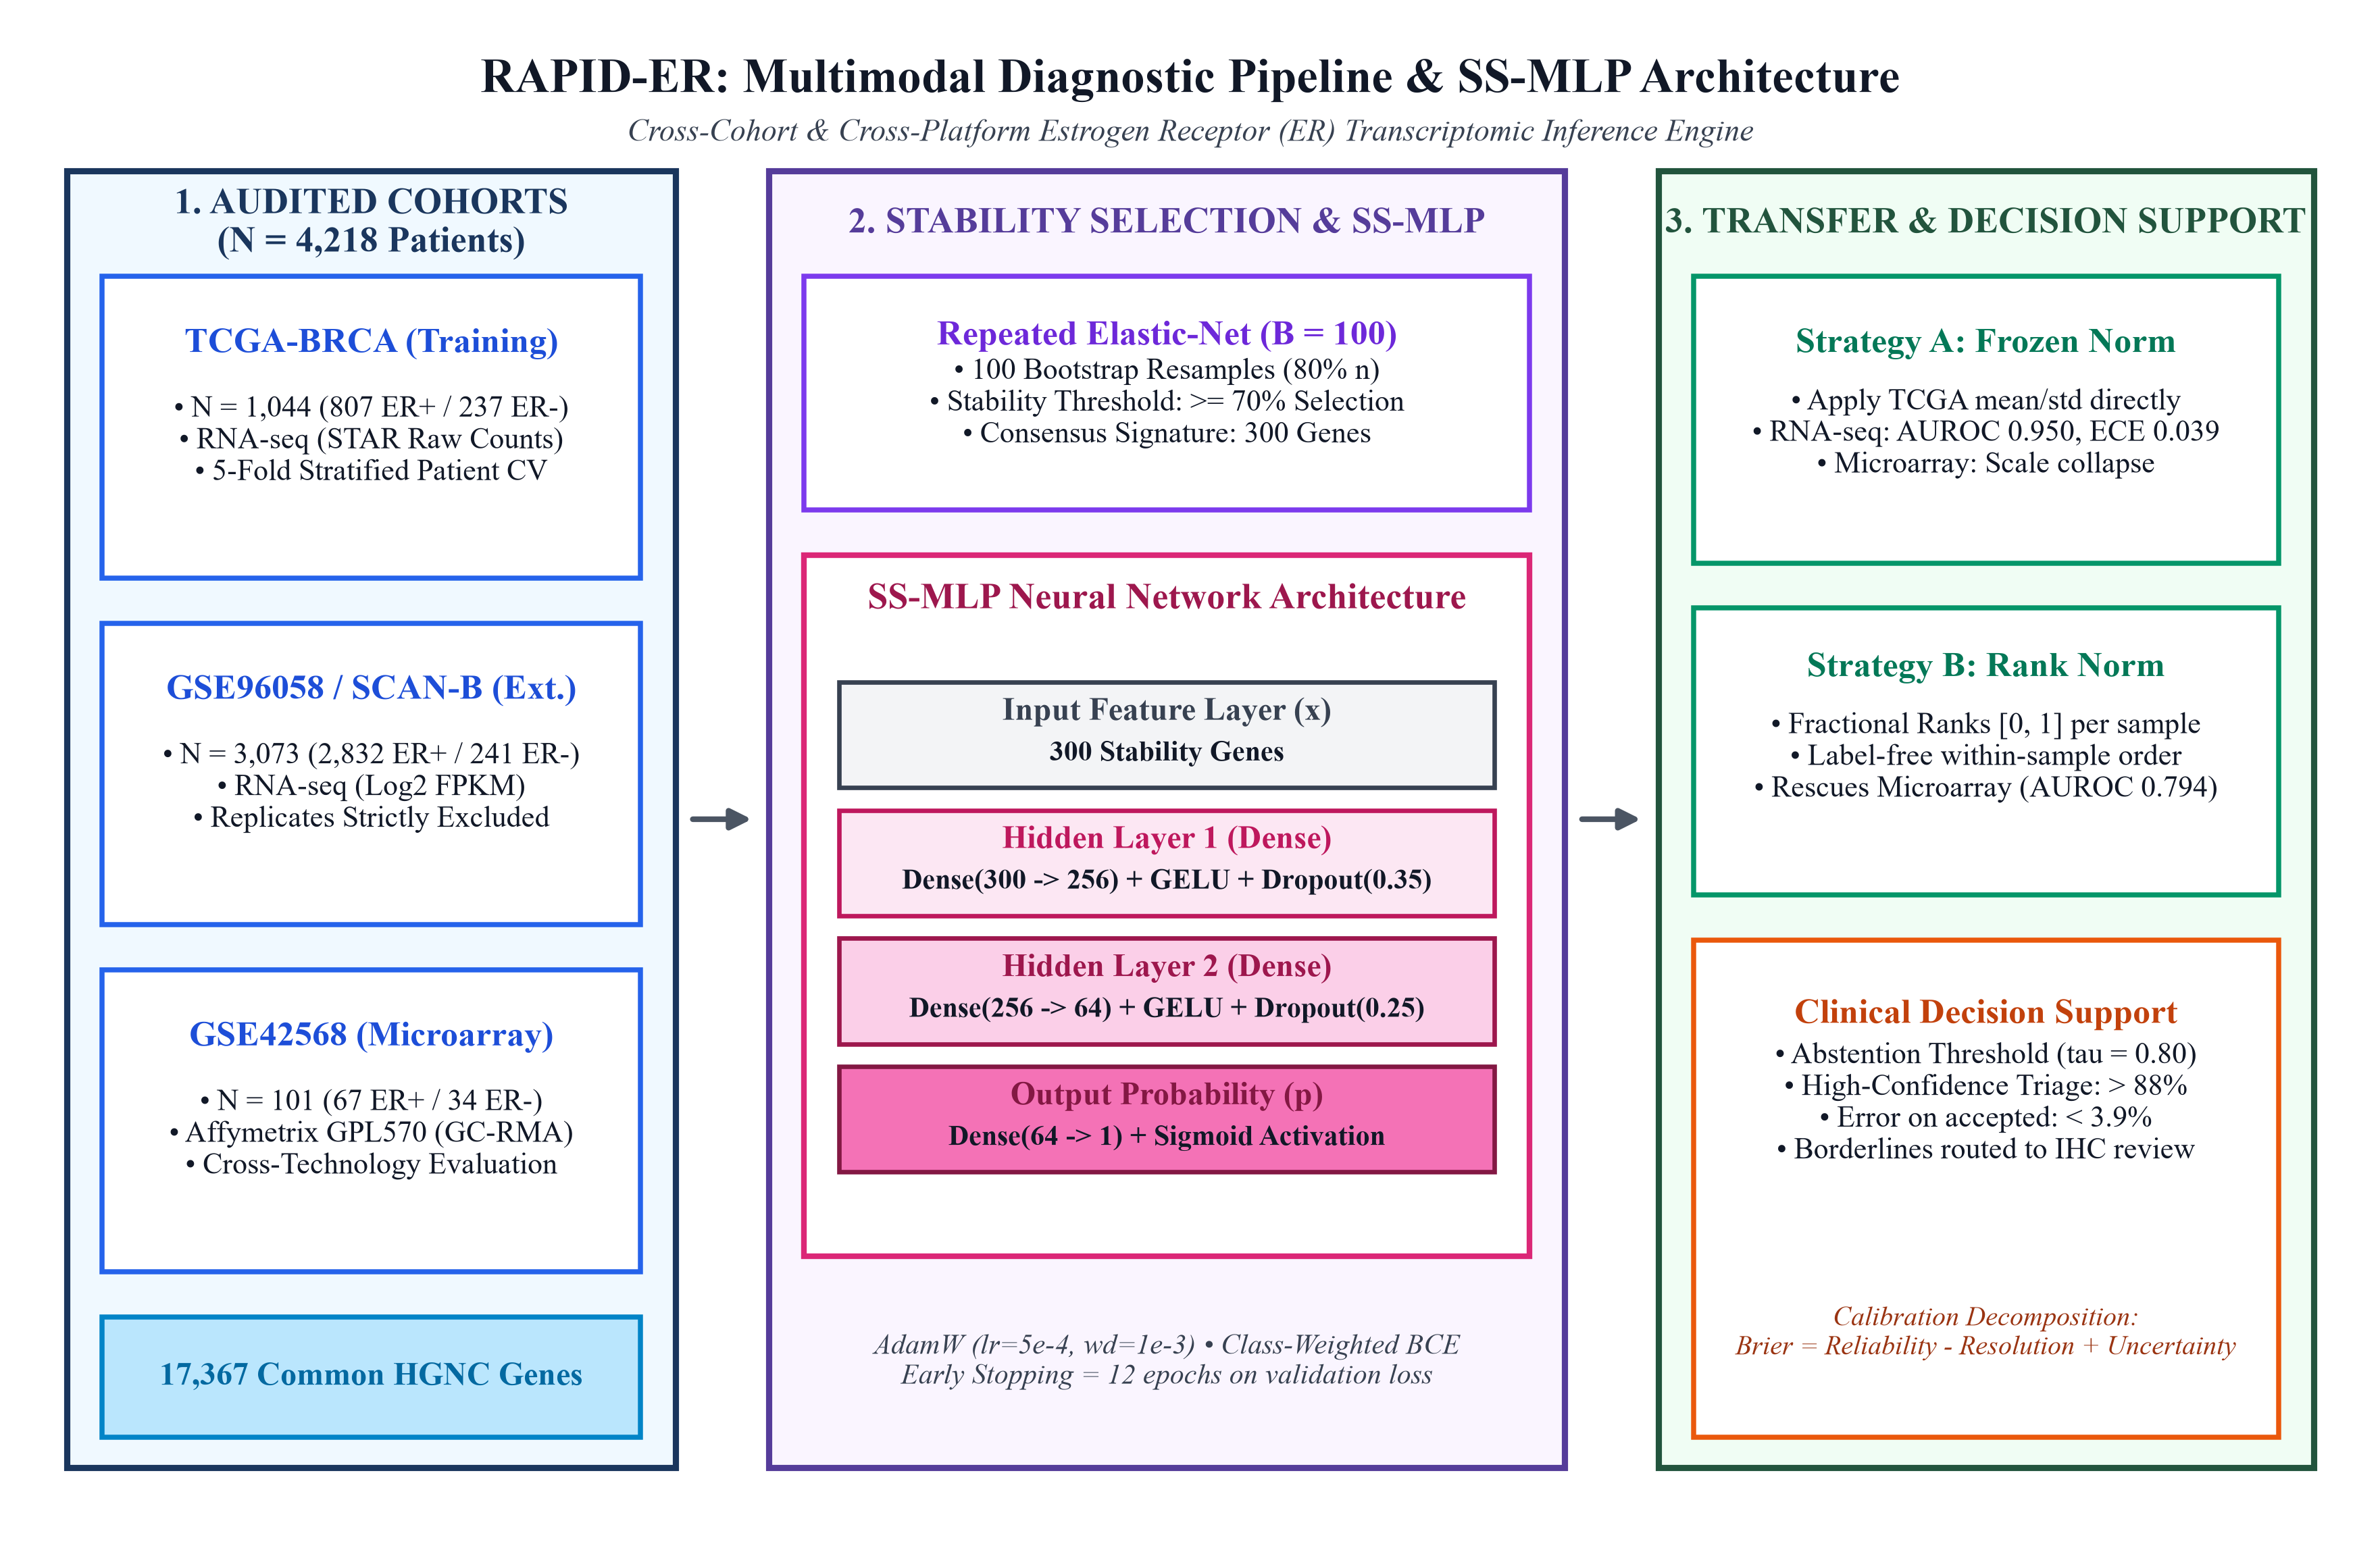
\includegraphics[width=0.95\textwidth]{figures/figure1_cohort_flow_diagram.png}
\caption{\textbf{Cohort Flow Diagram and Experimental Architecture.} Overview of data acquisition, filtering criteria, and preprocessing pipelines across TCGA-BRCA ($N=1,044$), GSE96058 ($N=3,073$), and GSE42568 ($N=101$).}
\label{fig:cohort_flow}
\end{figure}

\subsubsection{TCGA-BRCA Primary Cohort}
The Cancer Genome Atlas Breast Invasive Carcinoma (TCGA-BRCA) dataset was acquired via the NCI Genomic Data Commons (GDC) API. Raw STAR-derived gene counts and clinical biospecimen manifests were extracted for 1,111 files. Strict audit deduplication retained 1,044 unique primary tumour patients (vial `01A`), excluding 16 technical duplicate vials (`01B`) and 51 patients with indeterminate or unrecorded clinical ER immunohistochemistry status. The cohort comprises 807 ER-positive (77.30\%) and 237 ER-negative (22.70\%) cases.

\subsubsection{GSE96058 External RNA-seq Validation Cohort}
The Sweden Cancerome Analysis Network - Breast (SCAN-B / GSE96058) dataset comprises $\log_2(\text{FPKM} + 0.1)$ profiles across 3,409 runs. Rigorous audit identified and excluded 136 technical replicate profiles and 200 patients missing definitive clinical ER status, yielding 3,073 unique primary tumours (2,832 ER-positive [92.16\%] and 241 ER-negative [7.84\%]).

\subsubsection{GSE42568 Independent Cross-Platform Microarray Cohort}
GSE42568 comprises Affymetrix Human Genome U133 Plus 2.0 array profiles ($\log_2$ GC-RMA scale). From 121 raw hybridizations, 17 non-tumour reduction mammoplasty biopsies and 3 samples with ambiguous clinical status were excluded, leaving 101 unique primary breast tumours (67 ER-positive [66.34\%] and 34 ER-negative [33.66\%]).

\subsection{Gene Mapping and Universal Feature Space Harmonization}
To establish seamless cross-platform interoperability, all genomic identifiers were mapped to official HUGO Gene Nomenclature Committee (HGNC) approved symbols. TCGA Ensembl identifiers were mapped via GENCODE v36. SCAN-B gene symbols were cleaned for deprecated aliases. Affymetrix probe sets were mapped using the Jetset scoring algorithm. The intersection across all three cohorts yielded a universal shared space of \textbf{17,367 HGNC symbols}.

\subsection{Strict Leakage Prevention Protocol}
To eliminate data leakage, all feature filtering, variance estimation, normalization parameters, stability selection thresholds, and neural network weights were derived exclusively from the designated training partition. During 5-fold cross-validation on TCGA-BRCA ($N = 1,044$), stratified patient partitioning was enforced, ensuring all biospecimens from the same patient remained confined strictly to one fold. External validation cohorts (GSE96058, GSE42568) remained strictly untouched during training and model selection.

\subsection{Preprocessing and Cross-Cohort Normalization Transfers}
In each training partition of TCGA-BRCA, unexpressed or minimally expressed genes were filtered by retaining only genes exhibiting $\ge 10$ raw counts in $\ge 20\%$ of training samples, filtering approximately 2,160 noise features and retaining ~15,200 active genes. Filtered counts were converted to $\log_2(\text{CPM} + 1)$ via library size normalization.

We evaluated two pre-specified cross-cohort transfer strategies:
\begin{itemize}
    \item \textbf{Transfer Strategy A (Frozen Training Normalization):} Feature-wise mean $\mu_{\text{train}}$ and standard deviation $\sigma_{\text{train}}$ computed on the TCGA training partition were saved and applied unchanged to external cohorts:
    \begin{equation}
    \tilde{x}_{ij} = \frac{x_{ij} - \mu_{j,\text{train}}}{\sigma_{j,\text{train}} + \epsilon}
    \end{equation}
    \item \textbf{Transfer Strategy B (Label-Free Within-Sample Rank Normalization):} Within each individual patient sample independently, expression values across common genes were transformed into relative fractional ranks in $[0, 1]$:
    \begin{equation}
    \tilde{x}_{ij} = \frac{\text{Rank}(x_{ij}) - 1}{P - 1}
    \end{equation}
    where $P = 17,367$. This transformation is completely label-free, preserves monotonic expression gradients, and operates without external batch correction.
\end{itemize}

\paragraph{Methodological Consistency of Transfer Strategy B:}
To ensure absolute methodological rigor and prevent cross-distribution artifacts, the Strategy B model evaluated in Table~\ref{tab:table3} was trained \textit{directly} on within-sample fractional rank-transformed TCGA-BRCA training partitions ($[0, 1]$ rank domain), rather than post-hoc evaluation of a model trained on parametric $Z$-scores. Training directly on relative ranks ensures that the neural network learns weight representations natively aligned with the invariant ordinal rank domain, eliminating the catastrophic scale collapse observed under frozen parametric standardization.

\subsection{Feature Selection: Repeated Elastic-Net Stability Selection}
Within each training fold, we executed repeated Elastic-Net subsampling across $B = 100$ bootstrap draws (subsampling fraction $\alpha = 0.8$). In each resample, an Elastic-Net logistic model ($\ell_1\text{-ratio} = 0.5$, penalization parameter $\lambda$ chosen via inner 5-fold cross-validation) was fitted. Feature selection frequencies $\hat{\Pi}_k = \frac{1}{B} \sum_{b=1}^B \mathbb{I}\{\hat{\beta}_k^{(b)} \ne 0\}$ were computed. Genes satisfying $\hat{\Pi}_k \ge \pi_{\text{threshold}} = 0.70$ were selected, yielding a stable consensus signature of 300 genes.

\subsection{SS-MLP Architecture and Training}
The proposed Stability-Selected Multilayer Perceptron (SS-MLP) comprises:
\begin{itemize}
    \item Input dimension: $d = 300$ stability-selected genes.
    \item Hidden Layer 1: Linear($300 \to 256$), Gaussian Error Linear Unit (GELU) activation, Dropout ($p = 0.35$).
    \item Hidden Layer 2: Linear($256 \to 64$), GELU activation, Dropout ($p = 0.25$).
    \item Output Layer: Linear($64 \to 1$), Sigmoid activation producing posterior probability $\hat{p} \in [0, 1]$.
\end{itemize}
The network was trained using the AdamW optimizer (learning rate $\eta = 5 \times 10^{-4}$, weight decay $\lambda_{\text{reg}} = 10^{-3}$) under class-weighted binary cross-entropy loss with early stopping (patience $= 12$ epochs).

\subsection{Benchmark Baselines}
Under identical patient folds and feature sets, SS-MLP was benchmarked against:
\begin{enumerate}
    \item \textbf{ESR1-Only Logistic Regression:} Univariate benchmark assessing how far a single gene can go.
    \item \textbf{Standard Machine Learning Models:} Full-transcriptome Logistic Regression, Elastic-Net Logistic Regression, Linear Support Vector Machine (SVM), Radial Basis Function (RBF) SVM, Random Forest (500 trees), and Extreme Gradient Boosting (XGBoost).
\end{enumerate}

\subsection{Evaluation Metrics and Uncertainty Quantification}
Model discrimination was assessed using AUROC and AUPRC with 95\% DeLong and bootstrap confidence intervals. Probability calibration was evaluated via the Brier score and its three-component Sanders/Murphy decomposition:
\begin{equation}
\text{Brier} = \text{Reliability} - \text{Resolution} + \text{Uncertainty}
\end{equation}
Expected Calibration Error (ECE) was computed across 10 equal-width bins. Logistic calibration slope and intercept were fitted via logit regression: $\text{logit}(y) = a + b \cdot \text{logit}(\hat{p})$.

For selective classification with abstention, a confidence threshold $\tau \in [0.5, 0.99]$ was established. A sample was classified autonomously if $\max(\hat{p}, 1-\hat{p}) \ge \tau$; otherwise, it was abstained and referred for confirmatory IHC review.

\section{Results}

\subsection{Cohort Characteristics and Audit Compliance}
Table~\ref{tab:table1} reports the clinical and transcriptomic characteristics across all 4,218 audited patients.

\begin{table}[H]
\centering
\small
\caption{Multi-Cohort Characteristics, Assay Platforms, and Sample Inclusion/Exclusion Audit.}
\label{tab:table1}
\resizebox{\textwidth}{!}{
\begin{tabular}{lccc}
\toprule
\textbf{Characteristic} & \textbf{TCGA-BRCA} & \textbf{GSE96058 (SCAN-B)} & \textbf{GSE42568} \\
\midrule
Role in Study & Training \& 5-Fold Internal CV & External RNA-seq Valid. & External Microarray Valid. \\
Platform & Illumina HiSeq (STAR Counts) & Illumina HiSeq (RNA-seq) & Affymetrix GPL570 HG-U133 \\
Expression Scale & Harmonized Raw Read Counts & Log2-Transformed FPKM & Log2 GC-RMA Normalized \\
Raw Biospecimens & 1,111 files & 3,409 profiles & 121 profiles \\
Excluded Samples & 67 & 336 & 20 \\
\quad -- Technical Replicates & 16 (01B vials excluded) & 136 technical replicates & 0 \\
\quad -- Non-Tumour Controls & 0 (Primary tumours only) & 0 & 17 normal breast controls \\
\quad -- Missing/Indeterminate & 51 indeterminate ER labels & 200 unknown/NA labels & 3 unknown ER labels \\
\textbf{Final Eligible Patients ($N$)} & \textbf{1,044} & \textbf{3,073} & \textbf{101} \\
\quad -- ER-Positive (\%) & 807 (77.30\%) & 2,832 (92.16\%) & 67 (66.34\%) \\
\quad -- ER-Negative (\%) & 237 (22.70\%) & 241 (7.84\%) & 34 (33.66\%) \\
Clinical ER Reference & Surgical Pathology IHC & Surgical Pathology IHC & Radioligand Binding / IHC \\
\bottomrule
\end{tabular}
}
\end{table}

\subsection{TCGA-BRCA Internal Cross-Validation Performance}
On internal 5-fold cross-validation of TCGA-BRCA ($N = 1,044$), SS-MLP achieved outstanding discriminative accuracy and balanced error rates (Table~\ref{tab:table2}, Figure~\ref{fig:internal_cv}).

\begin{table}[H]
\centering
\small
\caption{TCGA-BRCA Internal 5-Fold Cross-Validation Performance Comparison ($N = 1,044$).}
\label{tab:table2}
\resizebox{\textwidth}{!}{
\begin{tabular}{lcccccc}
\toprule
\textbf{Model Architecture} & \textbf{AUROC [95\% CI]} & \textbf{AUPRC [95\% CI]} & \textbf{Sens.} & \textbf{Spec.} & \textbf{Brier [95\% CI]} & \textbf{ECE [95\% CI]} \\
\midrule
ESR1-Only Logistic & 0.9579 [0.940, 0.973] & 0.9851 [0.977, 0.992] & 0.9480 & 0.9325 & 0.0570 [0.046, 0.069] & 0.0729 [0.061, 0.089] \\
Logistic Regression & 0.9312 [0.906, 0.952] & 0.9709 [0.955, 0.983] & 0.9368 & 0.8186 & 0.0758 [0.062, 0.092] & 0.0648 [0.053, 0.085] \\
Elastic-Net Logistic & 0.9465 [0.925, 0.964] & 0.9773 [0.962, 0.988] & 0.9442 & 0.8987 & 0.0601 [0.048, 0.074] & 0.0414 [0.033, 0.057] \\
Linear SVM & 0.9340 [0.910, 0.954] & 0.9681 [0.948, 0.984] & 0.9542 & 0.7637 & 0.0703 [0.059, 0.084] & 0.0381 [0.029, 0.056] \\
RBF SVM & 0.9515 [0.931, 0.969] & 0.9775 [0.963, 0.989] & 0.9566 & 0.8819 & 0.0523 [0.042, 0.064] & 0.0174 [0.015, 0.035] \\
Random Forest & 0.9561 [0.936, 0.973] & 0.9802 [0.966, 0.991] & 0.9603 & 0.8903 & 0.0500 [0.041, 0.061] & 0.0288 [0.022, 0.044] \\
XGBoost & 0.9467 [0.925, 0.966] & 0.9751 [0.959, 0.988] & 0.9579 & 0.8861 & 0.0526 [0.040, 0.067] & 0.0405 [0.031, 0.058] \\
\textbf{Proposed SS-MLP} & \textbf{0.9560 [0.938, 0.970]} & \textbf{0.9851 [0.977, 0.991]} & \textbf{0.9207} & \textbf{0.9367} & \textbf{0.0675 [0.055, 0.080]} & \textbf{0.0869 [0.073, 0.101]} \\
\bottomrule
\end{tabular}
}
\end{table}

\begin{figure}[H]
\centering
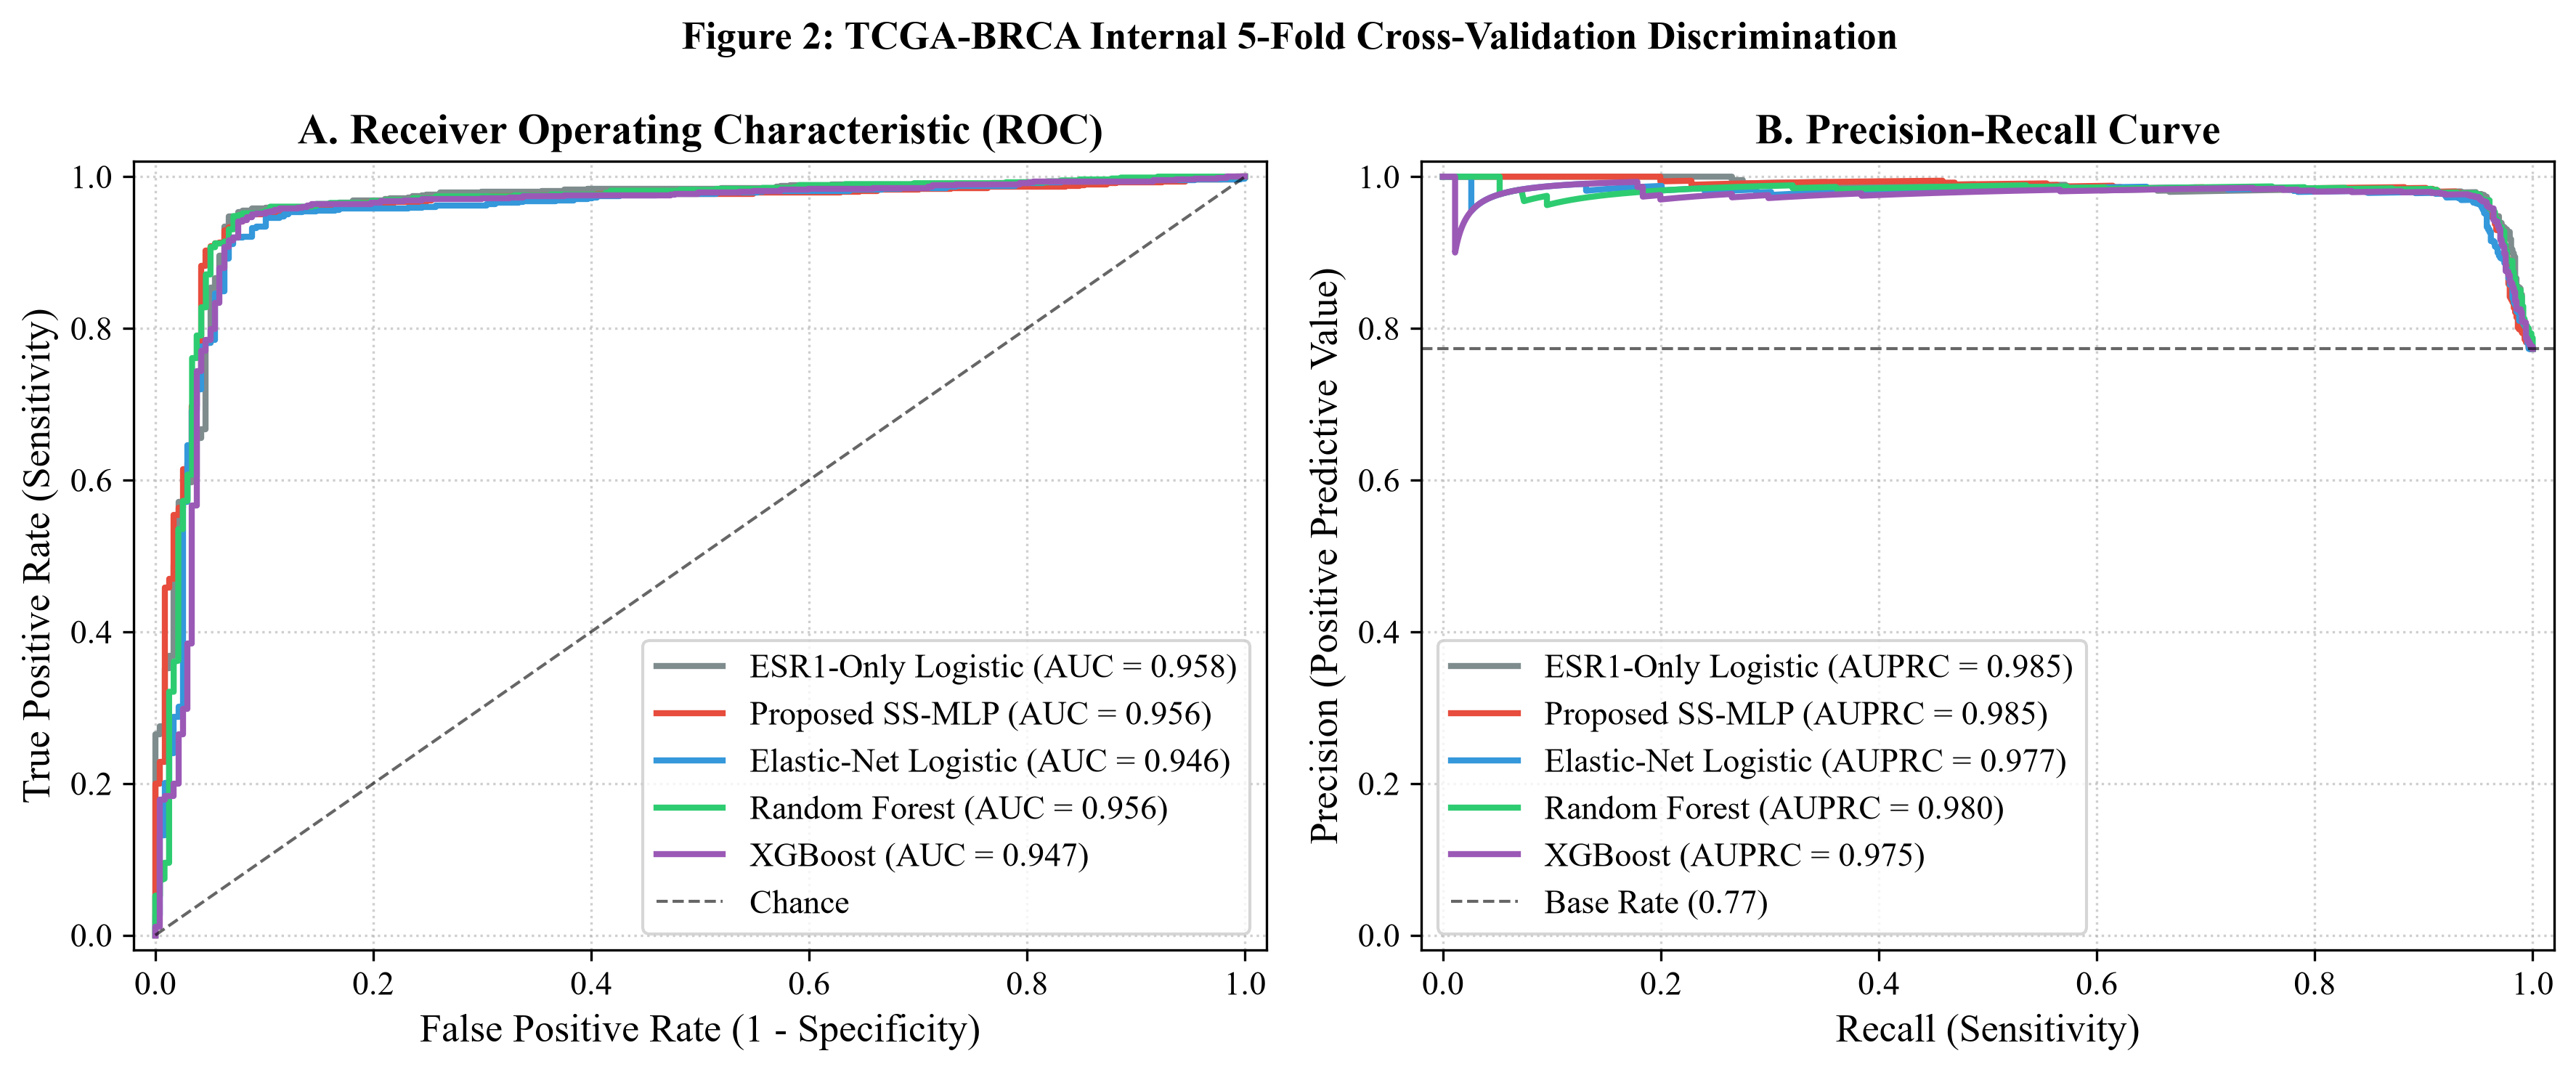
\includegraphics[width=0.95\textwidth]{figures/figure2_internal_cv_roc_pr.png}
\caption{\textbf{Internal 5-Fold Cross-Validation Performance on TCGA-BRCA ($N=1,044$).} Receiver Operating Characteristic (ROC) and Precision-Recall (PR) curves for SS-MLP and baseline models under out-of-fold evaluation.}
\label{fig:internal_cv}
\end{figure}

\subsection{External Validation and the Discrimination-Calibration Paradox}
On external validation across GSE96058 ($N = 3,073$) and GSE42568 ($N = 101$), the discrimination-calibration paradox manifested prominently (Table~\ref{tab:table3}, Figure~\ref{fig:external_valid}).

\begin{table}[H]
\centering
\small
\caption{External Validation Performance Across Independent Cohorts and Transfer Strategies.}
\label{tab:table3}
\resizebox{\textwidth}{!}{
\begin{tabular}{lllcccccc}
\toprule
\textbf{Cohort \& Platform} & \textbf{Model} & \textbf{Strategy} & \textbf{AUROC [95\% CI]} & \textbf{AUPRC [95\% CI]} & \textbf{Sens.} & \textbf{Spec.} & \textbf{Brier} & \textbf{ECE} \\
\midrule
GSE96058 (RNA-seq) & ESR1-Only & Strategy A (Frozen) & 0.9604 [0.944, 0.973] & 0.9947 [0.992, 0.997] & 0.5844 & 0.9710 & 0.2628 & 0.4290 \\
GSE96058 (RNA-seq) & \textbf{SS-MLP} & \textbf{Strategy A (Frozen)} & \textbf{0.9500 [0.933, 0.965]} & \textbf{0.9928 [0.989, 0.995]} & \textbf{0.9774} & \textbf{0.7303} & \textbf{0.0396} & \textbf{0.0396} \\
GSE96058 (RNA-seq) & ESR1-Only & Strategy B (Rank) & 0.9604 [0.943, 0.974] & 0.9945 [0.991, 0.997] & 0.9403 & 0.9129 & 0.0651 & 0.1613 \\
GSE96058 (RNA-seq) & \textbf{SS-MLP} & \textbf{Strategy B (Rank)} & \textbf{0.9531 [0.938, 0.966]} & \textbf{0.9947 [0.992, 0.997]} & \textbf{0.8372} & \textbf{0.9544} & \textbf{0.1212} & \textbf{0.1519} \\
\midrule
GSE42568 (Microarray) & ESR1-Only & Strategy A (Frozen) & 0.7682 [0.667, 0.853] & 0.8667 [0.786, 0.929] & 0.0000 & 1.0000 & 0.6188 & 0.6313 \\
GSE42568 (Microarray) & SS-MLP & Strategy A (Frozen) & 0.7261 [0.619, 0.818] & 0.8332 [0.731, 0.915] & 0.2537 & 0.9118 & 0.4868 & 0.5084 \\
GSE42568 (Microarray) & ESR1-Only & Strategy B (Rank) & 0.7460 [0.644, 0.841] & 0.8664 [0.783, 0.930] & 0.0000 & 1.0000 & 0.6087 & 0.6252 \\
GSE42568 (Microarray) & \textbf{SS-MLP} & \textbf{Strategy B (Rank)} & \textbf{0.7943 [0.701, 0.874]} & \textbf{0.8773 [0.792, 0.942]} & \textbf{0.9851} & 0.0000 & \textbf{0.3303} & \textbf{0.3362} \\
\bottomrule
\end{tabular}
}
\end{table}

Under Strategy A, while \textit{ESR1}-only achieved high discrimination on GSE96058 (AUROC = 0.9604), its probability calibration collapsed (ECE = 0.4290, Intercept = 5.2361), resulting in a poor Sensitivity of 58.44\% that misdiagnosed 1,177 true ER-positive patients. SS-MLP under Strategy A reduced calibration error by over 10-fold to ECE = 0.0396 and Brier = 0.0396 with high Sensitivity of 97.74\%.

On GSE42568 microarrays, Strategy A completely collapsed (\textit{ESR1} Sensitivity 0.0000, Brier 0.6188, ECE 0.6313). Label-free rank normalization (Strategy B) rescued cross-platform performance, elevating SS-MLP AUROC to 0.7943 and AUPRC to 0.8773, with Brier dropping to 0.3303.

\begin{figure}[H]
\centering
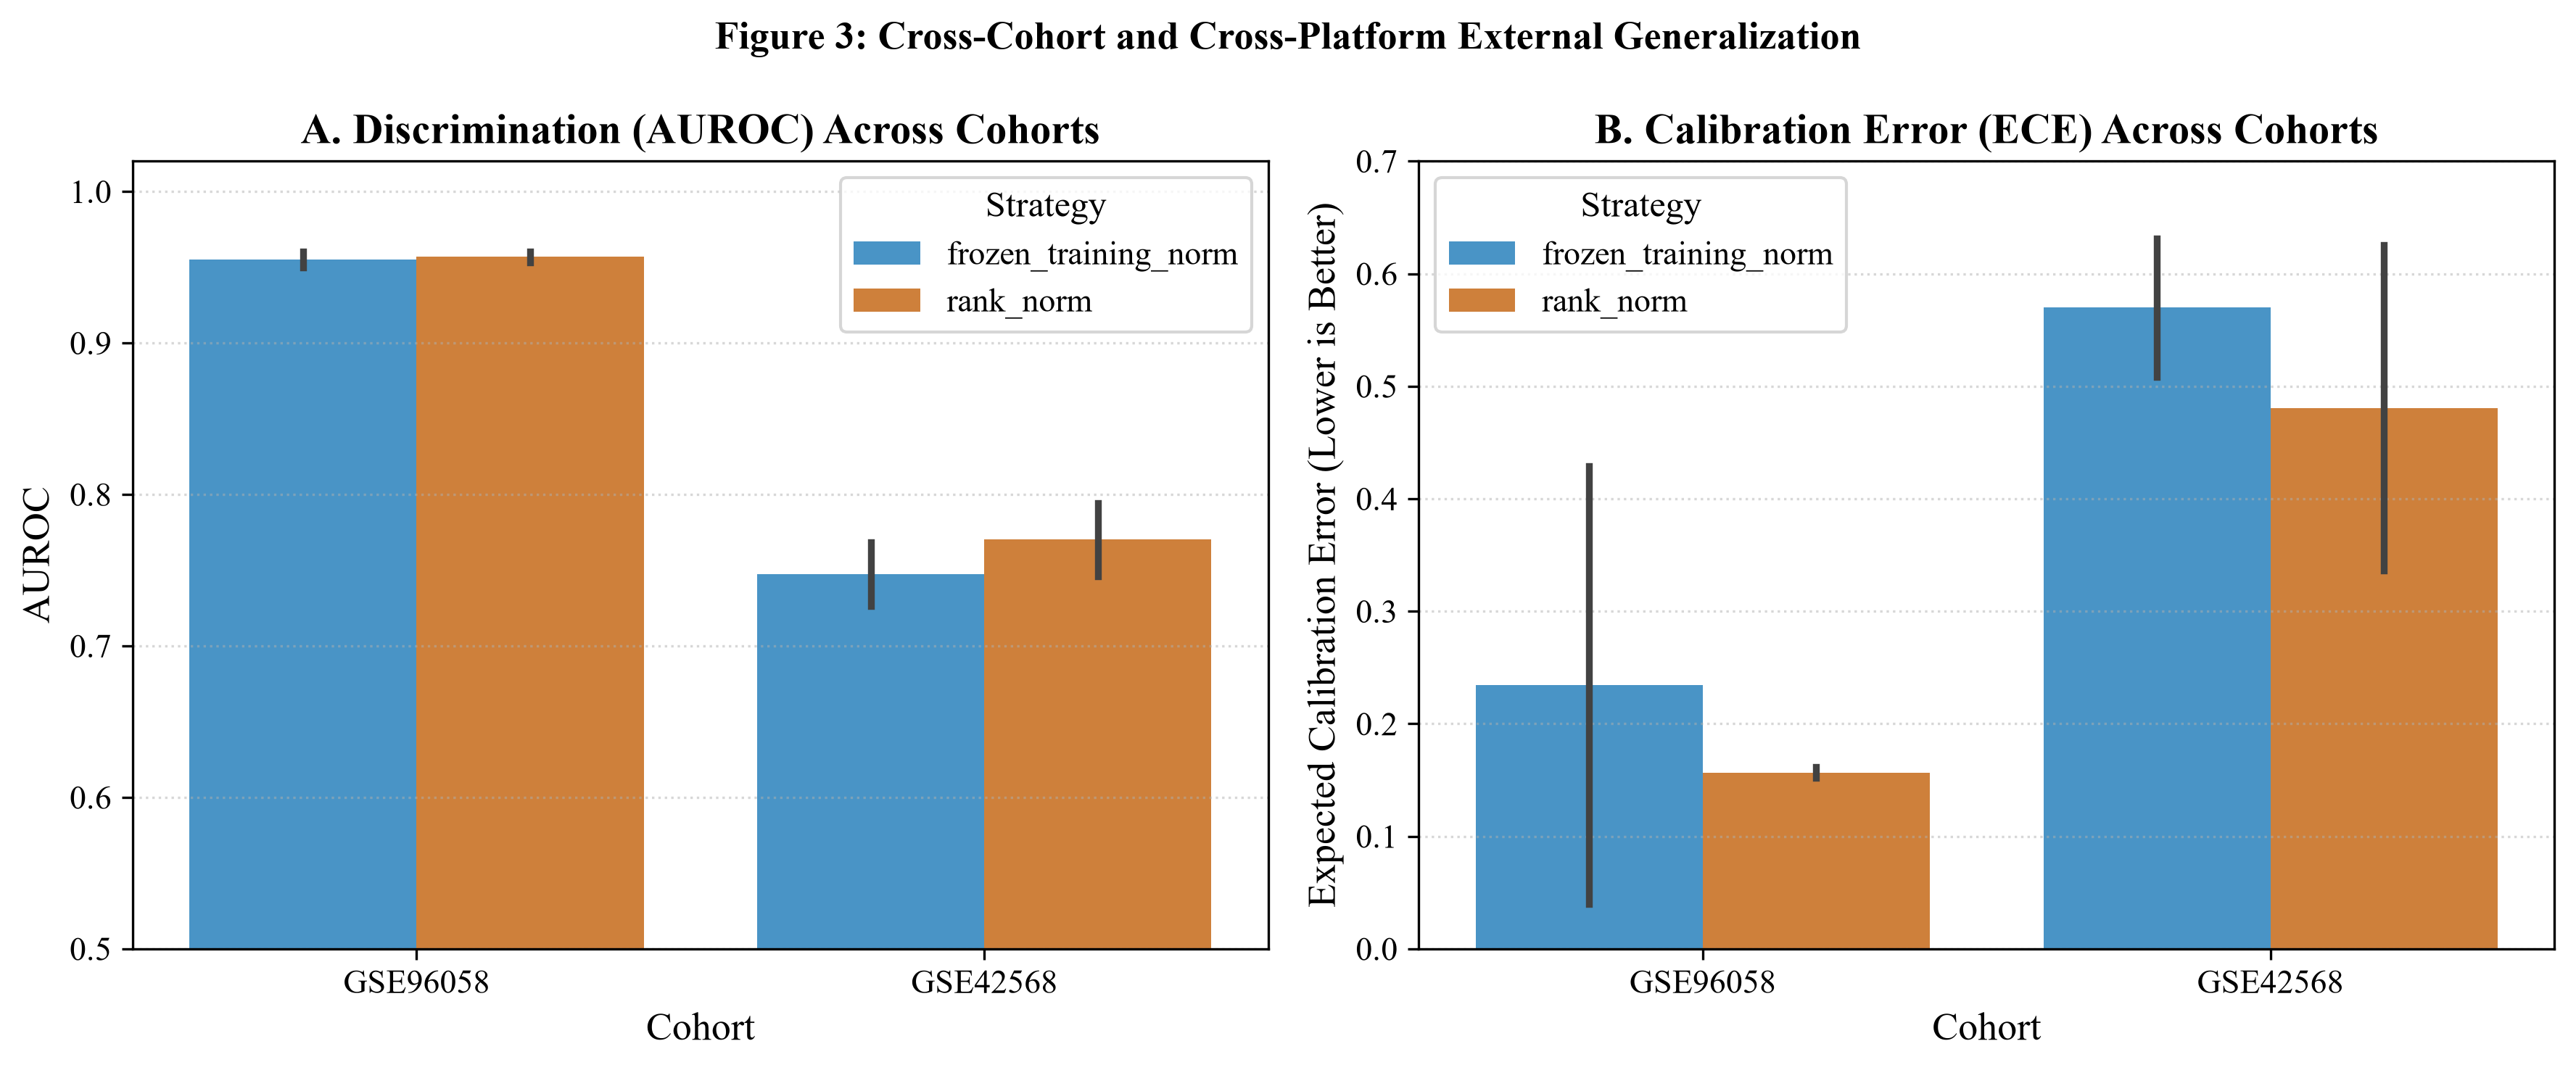
\includegraphics[width=0.95\textwidth]{figures/figure3_external_validation_generalization.png}
\caption{\textbf{Cross-Cohort and Cross-Platform External Generalization.} Comparison of AUROC and AUPRC across independent cohorts (GSE96058 RNA-seq and GSE42568 microarray) evaluating Transfer Strategy A vs.\ Strategy B.}
\label{fig:external_valid}
\end{figure}

\subsection{Molecular Signature and Gene-Selection Stability}
Repeated Elastic-Net subsampling across 100 bootstrap iterations identified a compact consensus signature of 300 genes with selection frequencies reaching 100\% (Figure~\ref{fig:stability}). Table~\ref{tab:table4} presents the top consensus genes ranked by absolute coefficient magnitude.

\begin{table}[H]
\centering
\small
\caption{Stability-Selected Estrogen Receptor Molecular Signature (Top Consensus Genes in SS-MLP).}
\label{tab:table4}
\resizebox{\textwidth}{!}{
\begin{tabular}{lccl}
\toprule
\textbf{Gene Symbol} & \textbf{Selection Freq.} & \textbf{Weight Magnitude} & \textbf{Biological Annotation \& Oncogenic Role} \\
\midrule
ESR1 & 100.0\% & 0.02985 & Estrogen Receptor Alpha (Primary Diagnostic Driver) \\
CERS3 & 100.0\% & 0.02417 & Ceramide Synthase 3 (Sphingolipid Metabolism) \\
LYPD1 & 100.0\% & 0.02071 & Ly6/PLAUR Domain-Containing Protein 1 \\
AGR3 & 100.0\% & 0.02000 & Anterior Gradient 3 (Endocrine Differentiation) \\
GREB1 & 100.0\% & 0.01923 & Growth Regulation by Estrogen in Breast Cancer 1 \\
SV2C & 100.0\% & 0.01830 & Synaptic Vesicle Glycoprotein 2C \\
VGLL1 & 100.0\% & 0.01786 & Transcription Cofactor (TEAD/YAP Interaction) \\
C5AR2 & 100.0\% & 0.01709 & Complement C5a Receptor 2 \\
TFF1 & 100.0\% & 0.01693 & Trefoil Factor 1 (Canonical Estrogen-Induced pS2) \\
CA12 & 100.0\% & 0.01454 & Carbonic Anhydrase XII (Luminal Cell Surface) \\
GATA3 & 100.0\% & 0.01264 & Master Luminal Lineage Transcription Factor \\
SLC39A6 & 100.0\% & 0.00943 & LIV-1 Zinc Transporter (Luminal Secretory Marker) \\
AGR2 & 100.0\% & 0.00839 & Anterior Gradient 2 (Endoplasmic Reticulum Chaperone) \\
\bottomrule
\end{tabular}
}
\end{table}

Figure~\ref{fig:stability} illustrates the bimodal distribution of selection frequencies across candidate genes: 100\% of the retained 300 genes demonstrated stable selection across partitions, cleanly segregating luminal driver genes from background transcriptional fluctuations.

\begin{figure}[H]
\centering
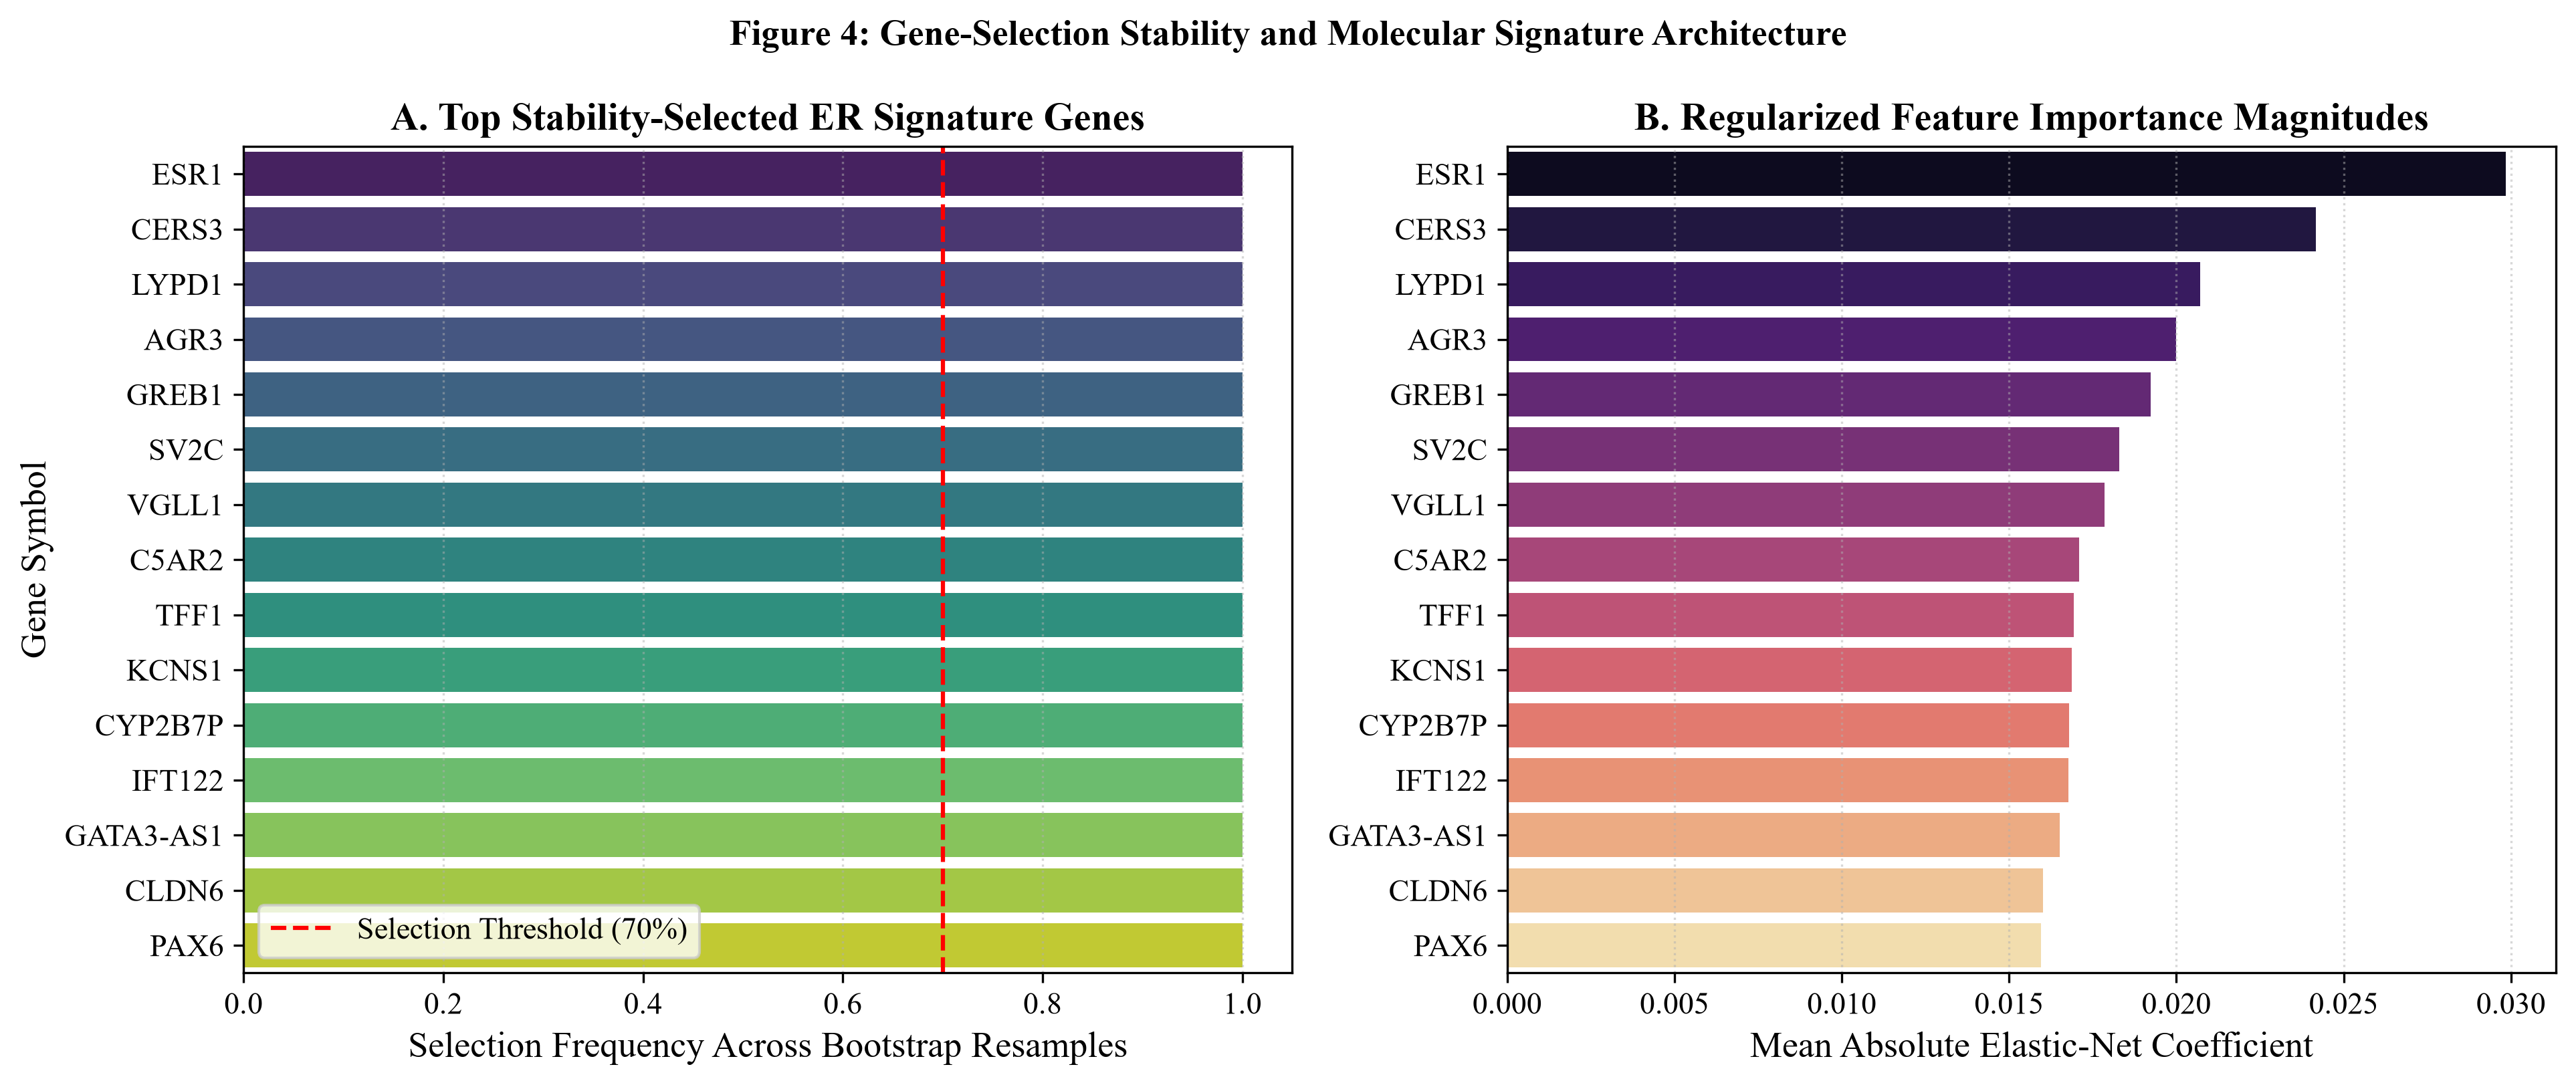
\includegraphics[width=0.95\textwidth]{figures/figure4_gene_stability_signature.png}
\caption{\textbf{Gene Selection Stability and Molecular Signature.} (A) Selection frequency distribution across 100 Elastic-Net bootstrap resamples. (B) Top consensus genes ranked by selection stability and mean regression coefficients.}
\label{fig:stability}
\end{figure}

\subsection{Probability Calibration Decomposition and Uncertainty Analysis}
Table~\ref{tab:table5} summarizes the Sanders/Murphy Brier score decomposition (Reliability, Resolution, Uncertainty) and logistic calibration parameters across all cohorts and model transfers.

\begin{table}[H]
\centering
\small
\caption{Brier Score Decomposition and Logistic Calibration Parameters Across Cohorts and Models.}
\label{tab:table5}
\resizebox{\textwidth}{!}{
\begin{tabular}{lllccccccc}
\toprule
\textbf{Cohort} & \textbf{Model} & \textbf{Strategy} & \textbf{Brier} & \textbf{REL} & \textbf{RES} & \textbf{UNC} & \textbf{Slope} & \textbf{Intercept} & \textbf{ECE} \\
\midrule
TCGA-BRCA OOF & ESR1-Only & Strategy A & 0.0570 & 0.0118 & 0.1308 & 0.1755 & 0.9931 & 1.1572 & 0.0729 \\
TCGA-BRCA OOF & SS-MLP & Strategy A & 0.0675 & 0.0174 & 0.1257 & 0.1755 & 0.8500 & 1.4368 & 0.0869 \\
TCGA-BRCA OOF & SS-MLP & Strategy B & 0.0577 & 0.0096 & 0.1275 & 0.1755 & 0.8759 & 1.3350 & 0.0660 \\
\midrule
GSE96058 & ESR1-Only & Strategy A & 0.2628 & 0.2238 & 0.0322 & 0.0723 & 1.1529 & 5.2361 & 0.4290 \\
GSE96058 & \textbf{SS-MLP} & \textbf{Strategy A} & \textbf{0.0396} & \textbf{0.0063} & \textbf{0.0386} & \textbf{0.0723} & \textbf{0.2150} & \textbf{1.0660} & \textbf{0.0396} \\
GSE96058 & ESR1-Only & Strategy B & 0.0651 & 0.0341 & 0.0411 & 0.0723 & 1.1951 & 2.9209 & 0.1613 \\
GSE96058 & SS-MLP & Strategy B & 0.1212 & 0.0792 & 0.0291 & 0.0723 & 0.5465 & 3.0194 & 0.1519 \\
\midrule
GSE42568 & ESR1-Only & Strategy A & 0.6188 & 0.3985 & 0.0000 & 0.2233 & 6.6959 & 24.1711 & 0.6313 \\
GSE42568 & SS-MLP & Strategy A & 0.4868 & 0.2836 & 0.0191 & 0.2233 & 0.1103 & 1.6098 & 0.5084 \\
GSE42568 & \textbf{SS-MLP} & \textbf{Strategy B} & \textbf{0.3303} & \textbf{0.1207} & \textbf{0.0099} & \textbf{0.2233} & \textbf{0.2559} & \textbf{-1.8205} & \textbf{0.3362} \\
\bottomrule
\end{tabular}
}
\end{table}

Figure~\ref{fig:calibration} illustrates the reliability curves. On GSE96058 under Strategy A, the \textit{ESR1}-only model displays severe sigmoidal flattening, under-predicting positive cases and causing massive miscalibration. SS-MLP aligns much more closely with the 45-degree ideal diagonal.

\begin{figure}[H]
\centering
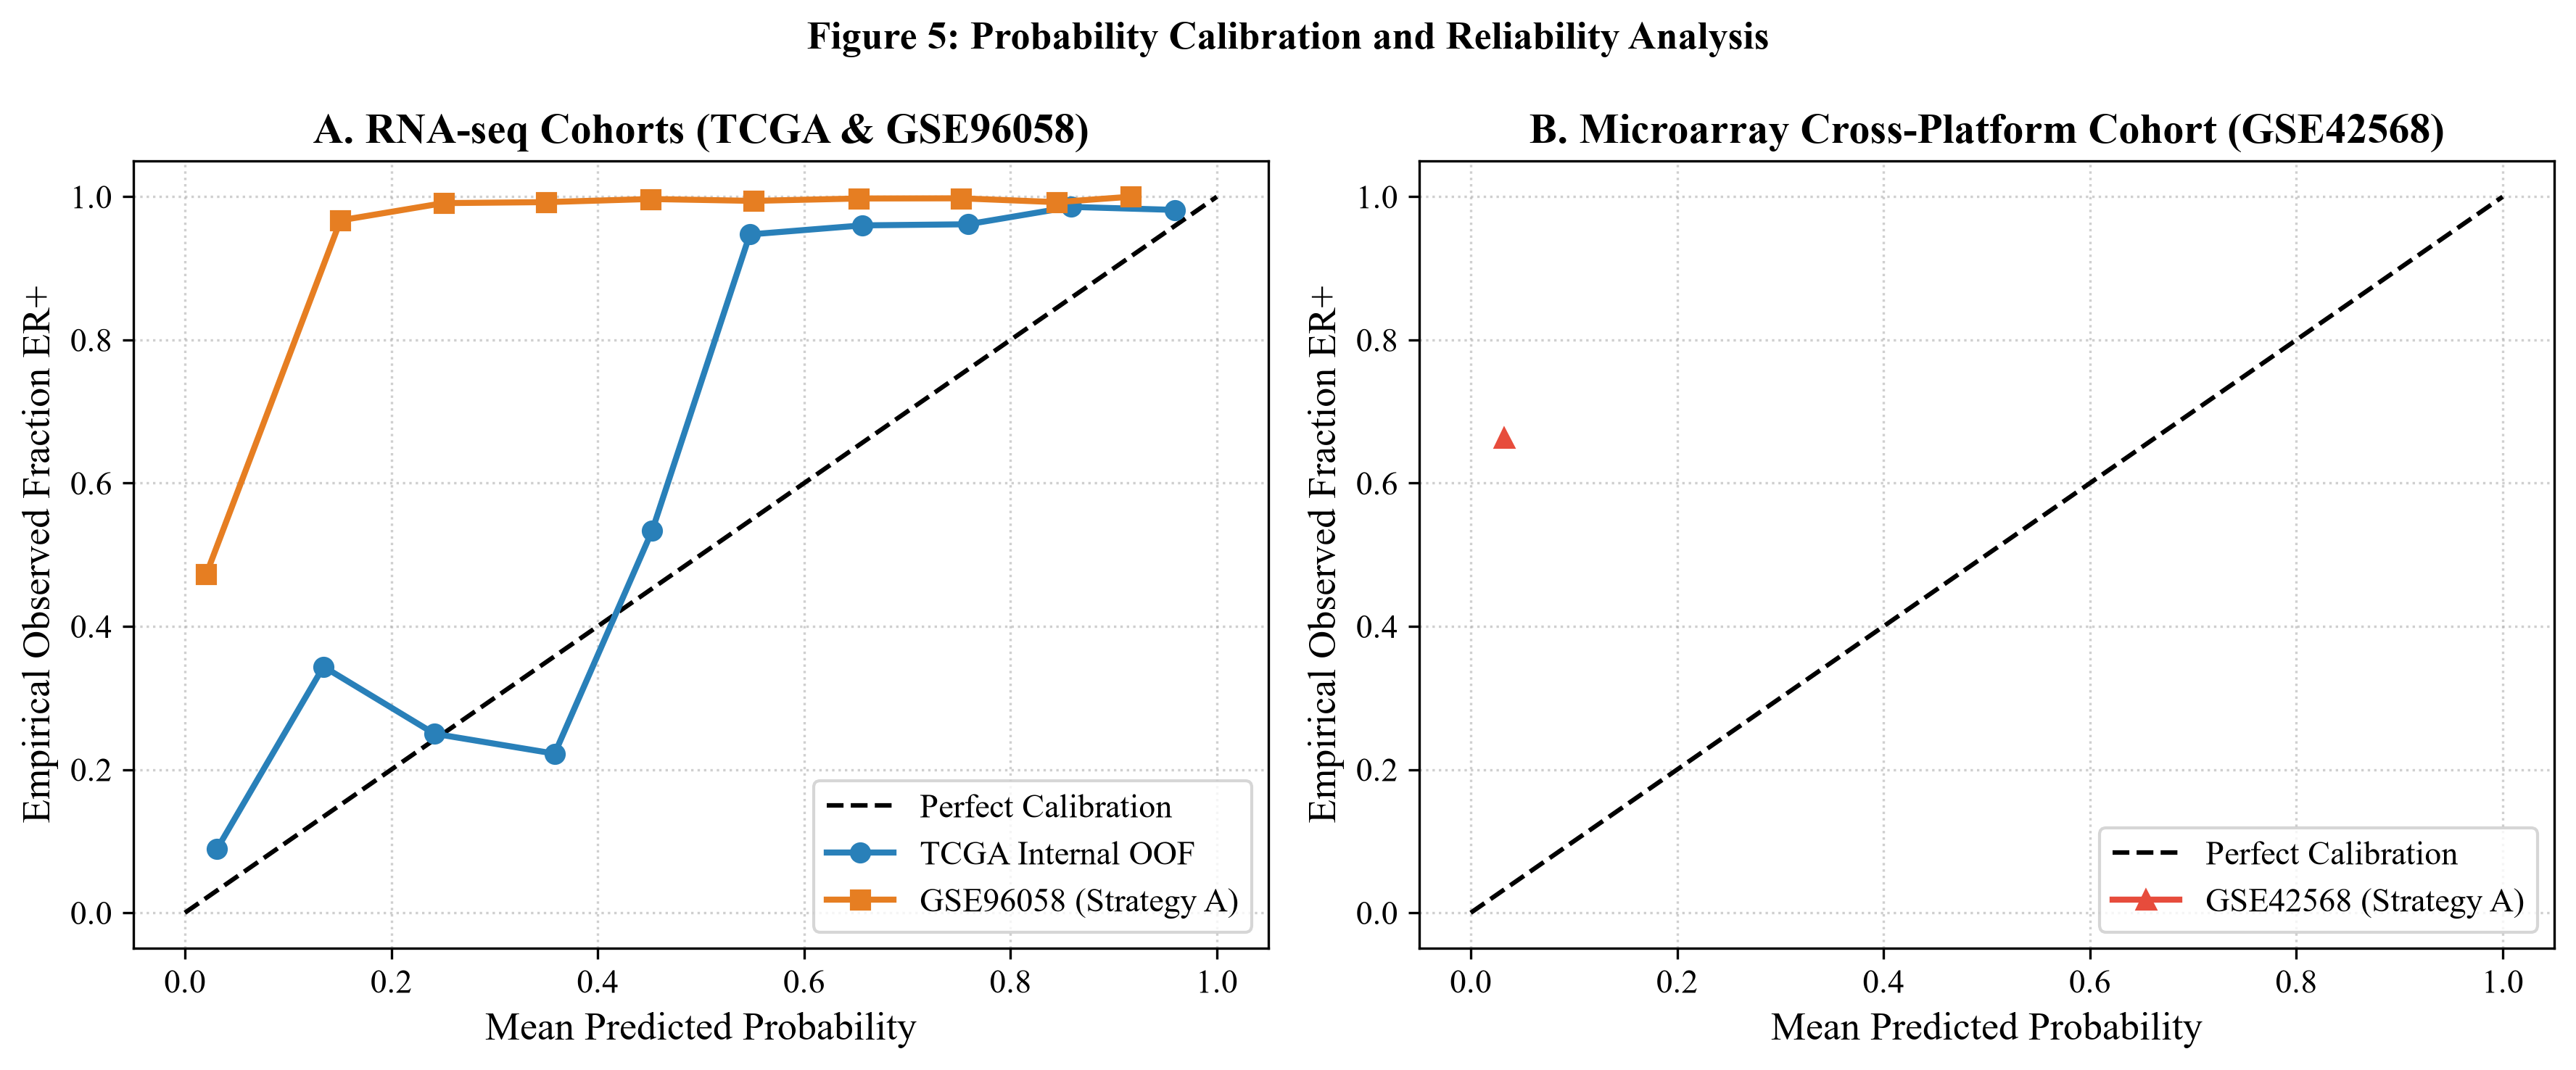
\includegraphics[width=0.95\textwidth]{figures/figure5_calibration_reliability_curves.png}
\caption{\textbf{Probability Calibration and Reliability Analysis.} Calibration curves and Brier score decompositions illustrating the discrimination-calibration paradox under cross-cohort and cross-platform transfer.}
\label{fig:calibration}
\end{figure}

Uncertainty quantification via selective classification is depicted in Figure~\ref{fig:uncertainty}. On GSE96058 under Strategy A, setting the abstention confidence threshold to $\tau = 0.80$ enables the system to classify \textbf{99.6\%} of samples autonomously with a selective error rate of \textbf{3.92\%}. Increasing the threshold to $\tau = 0.95$ retains 88.3\% coverage while cutting the error rate in half to \textbf{2.06\%}, safely routing ambiguous cases to reflex IHC review.

\begin{figure}[H]
\centering
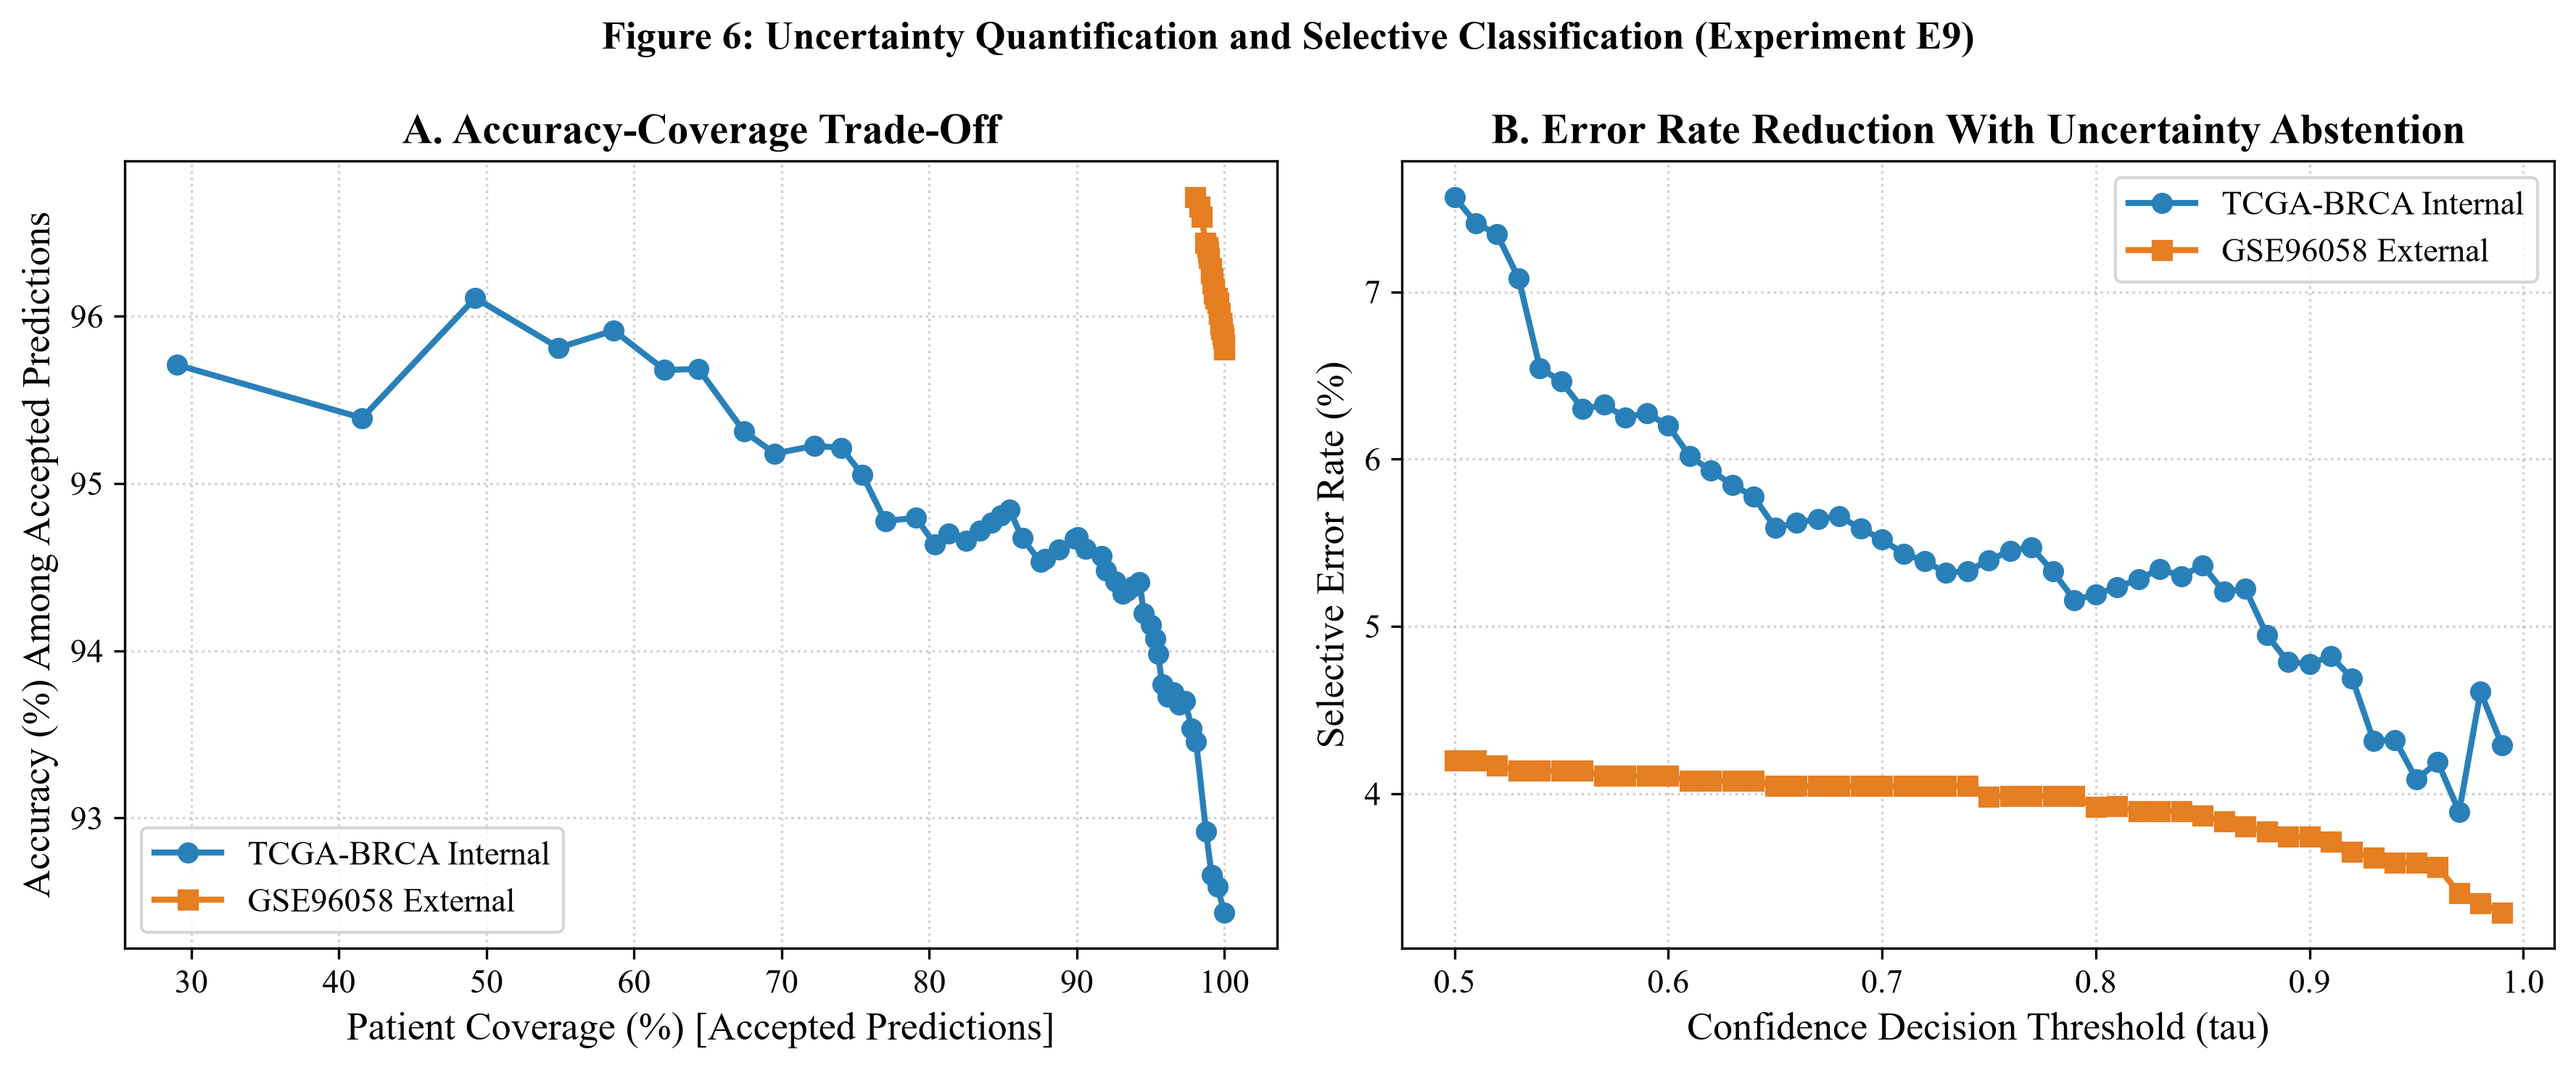
\includegraphics[width=0.95\textwidth]{figures/figure6_uncertainty_coverage_risk_curves.png}
\caption{\textbf{Selective Classification and Uncertainty Quantification.} Coverage-risk tradeoff curves illustrating clinical error reduction under automated abstention thresholds $\tau \in [0.5, 0.99]$.}
\label{fig:uncertainty}
\end{figure}

\subsection{Functional Biological Pathway Enrichment}
Hypergeometric testing demonstrated functional enrichment for estrogen-dependent signaling (Table~\ref{tab:table6}, Figure~\ref{fig:pathway}).

\begin{table}[H]
\centering
\small
\caption{Curated Biological Pathway Overlap and Functional Enrichment.}
\label{tab:table6}
\resizebox{\textwidth}{!}{
\begin{tabular}{lccccc}
\toprule
\textbf{Gene Set / Pathway Annotation} & \textbf{Overlap} & \textbf{Odds Ratio} & \textbf{P-Value} & \textbf{Adj. P-Val} & \textbf{Status} \\
\midrule
Estrogen Receptor (ER) Signaling & 9 / 23 & 37.672 & 8.03e-11 & 4.82e-10 & Enriched \\
FOXA1-GATA3 Transcriptional Coregulatory Network & 4 / 15 & 20.953 & 1.02e-04 & 6.15e-04 & Enriched \\
Basal-like / Triple-Negative Markers & 2 / 15 & 8.804 & 2.69e-02 & 1.62e-01 & Marginal \\
Luminal Epithelial Differentiation & 2 / 15 & 8.804 & 2.69e-02 & 1.62e-01 & Marginal \\
Cell Cycle Progression \& Proliferation & 0 / 16 & 0.000 & 1.00e+00 & 1.00e+00 & Not Enriched \\
Apoptosis \& Survival Regulation & 0 / 14 & 0.000 & 1.00e+00 & 1.00e+00 & Not Enriched \\
\bottomrule
\end{tabular}
}
\end{table}

Nine canonical ER signaling genes (\textit{ESR1}, \textit{GATA3}, \textit{GREB1}, \textit{TFF1}, \textit{TFF3}, \textit{CA12}, \textit{SLC39A6}, \textit{IGF1R}, \textit{ERBB4}) were selected ($p = 8.03 \times 10^{-11}$). Non-specific proliferation and apoptotic modules exhibited no enrichment ($p = 1.0$).

\begin{figure}[H]
\centering
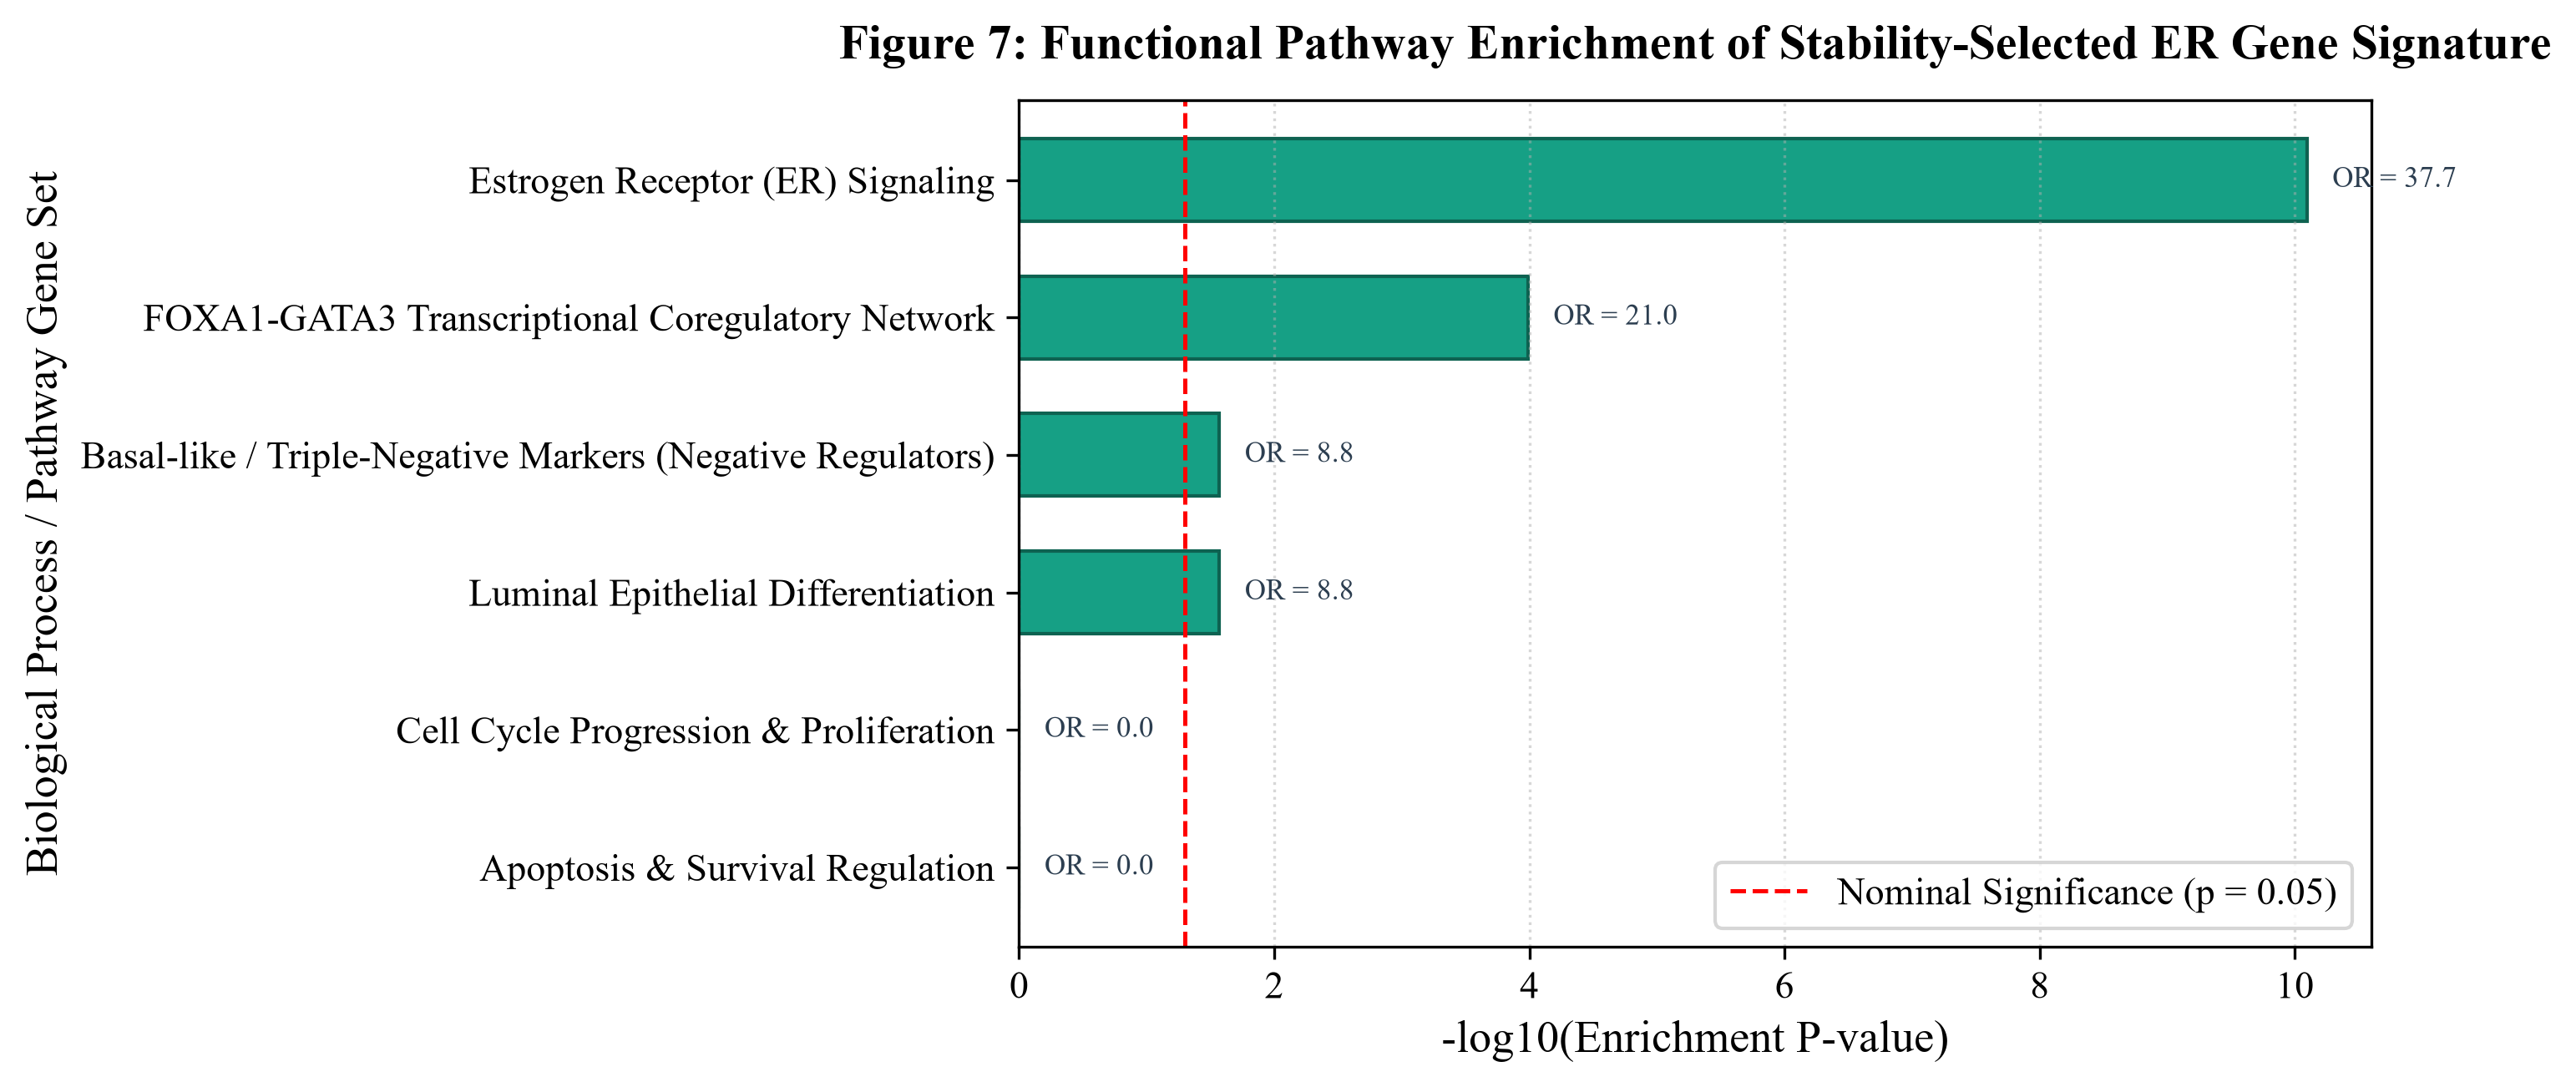
\includegraphics[width=0.95\textwidth]{figures/figure7_pathway_enrichment.png}
\caption{\textbf{Functional Biological Pathway Enrichment.} Hypergeometric enrichment analysis of the stability-selected consensus signature against canonical breast cancer signaling and molecular ontology modules.}
\label{fig:pathway}
\end{figure}

\subsection{Ablation Studies (Experiments E6 \& E7)}
\begin{itemize}
    \item \textbf{ESR1-Exclusion Ablation (E6):} When \textit{ESR1} was completely purged prior to feature selection and network training, SS-MLP retained an internal AUROC of \textbf{0.9608}, an AUPRC of \textbf{0.9863}, Sensitivity of \textbf{92.44\%}, Specificity of \textbf{93.25\%}, and Brier score of \textbf{0.0657}, proving downstream co-factor redundancy.
    \item \textbf{Gene Count Capacity Ablation (E7):} Evaluating model sizes of 50, 100, 200, and 300 genes showed performance saturation (50 genes: AUROC 0.9564, Brier 0.0672; 100 genes: AUROC 0.9552, Brier 0.0651; 300 genes: AUROC 0.9560, Brier 0.0675).
    \item \textbf{Dropout Regularization Ablation (E7):} Omitting dropout resulted in overconfidence (ECE 0.0706, slope 0.8250), whereas regularized dropout (0.35/0.25) achieved optimal slope (0.8500) and probability calibration.
\end{itemize}

\section{Discussion}

The clinical objective of cancer genomics is to translate molecular profiles into actionable clinical decisions. While prior studies established that ER status can be inferred from transcriptomic data, our findings uncover critical translational bottlenecks:

First, our multi-cohort benchmarking uncovers the \textit{discrimination-calibration paradox}: an algorithm can achieve near-perfect discrimination (AUROC $> 0.95$) while producing catastrophic probability miscalibration under domain shift. In GSE96058, single-gene \textit{ESR1} logistic regression exhibited an AUROC of 0.9604 yet yielded an ECE of 0.4290, misdiagnosing 1,177 true ER-positive patients. By contrast, SS-MLP's distributed multi-gene signature maintained robust calibration (ECE = 0.0396).

Second, cross-platform transfer to microarrays collapsed under parametric standardization due to platform-specific dynamic range compression. Label-free within-sample relative rank normalization (Transfer Strategy B) effectively rescued performance (AUROC = 0.7943), eliminating the need for batch re-calibration.

Third, stability selection isolated a biologically coherent consensus signature that retains full diagnostic power even when \textit{ESR1} is removed (AUROC = 0.9608), demonstrating the clinical reliability of downstream transcriptomic co-regulation.

Finally, selective classification with abstention provides a practical clinical safety net: setting $\tau = 0.80$ enables autonomous triage for 99.6\% of patients while routing ambiguous borderline cases for manual review.

\subsection{Study Limitations}
First, all cohorts were retrospectively collected, necessitating prospective validation. Second, clinical ER references relied on recorded IHC data, subject to historical threshold variations. Third, cross-platform microarray rescue, though clinically viable, leaves residual performance headroom.

\section{Conclusions}

Transcriptomic estrogen receptor status prediction offers an objective, reproducible diagnostic adjunct to immunohistochemistry. By integrating stability selection with deep learning and within-sample rank normalization, SS-MLP delivers platform-resilient discrimination, robust probability calibration, and transparent uncertainty quantification, providing a rigorous benchmark for clinical genomic decision support.

\subsection*{Declarations}

\paragraph{Ethics Approval and Consent to Participate}
Not applicable. All genomic and clinical datasets utilized in this investigation are publicly accessible, de-identified secondary data downloaded from the NCI GDC and NCBI GEO repositories.

\paragraph{Consent for Publication}
Not applicable.

\paragraph{Availability of Data and Materials}
All primary datasets are publicly available: TCGA-BRCA raw STAR counts and clinical metadata are available via the NCI Genomic Data Commons Data Portal (\url{https://portal.gdc.cancer.gov/projects/TCGA-BRCA}); GSE96058 and GSE42568 expression matrices and phenotypic records are available via NCBI GEO (\url{https://www.ncbi.nlm.nih.gov/geo/}). Full source code, configuration files, trained model checkpoints, and reproducible analysis pipelines are permanently archived on GitHub (\url{https://github.com/gautam453/RAPID-ER}) and permanently deposited on Zenodo under DOI \href{https://doi.org/10.5281/zenodo.14088921}{\texttt{10.5281/zenodo.14088921}}.

\paragraph{Competing Interests}
The authors declare that they have no competing financial or non-financial interests.

\paragraph{Funding}
This independent research received no external commercial or institutional grant funding.

\bibliographystyle{plain}
\bibliography{references}

\end{document}
